\chapter{Opis implementacji}
\label{cha:uzywaneTechnologie}

\section{Opis użytych technologii i narzędzi}
\label{sec:technology}
Przy implementacji pracy zostały użyte następujące technologie i narzędzia:
\begin{itemize}
\item Ruby on Rails - jest to framework webowy służący do tworzenia aplikacji internetowych. Został napisany w interpretowanym skryptowym języku Ruby. Ruby on Rails wpisuje się w architekturę Model View Controller (MVC), dostarczając podstawowe struktury dla bazy danych, serwisów oraz stron internetowych. Domyślnym formatem wymiany danych w tym frameworku jest JSON oraz XML. Przy wyświetlaniu stron zaleca się korzystanie z szablonów ERB lub HAML, JavaScript oraz SASS ( jest to język podobny do CSS cechujący się znacznie większą przejrzystością oraz mniejszą ilością kodu). Ruby on Rails w bardzo prosty sposób umożliwa dołączenie do aplikacji dodatkowych, gotowych bibliotek nazywanych gemami. Nadrzędnym celem twórców tego frameworku było wprowadzenie zasad DRY (Don't repeat yourself - Nie powtarzaj się) oraz CoC (Convention over Configuration - konwencja ponad konfiguracją). Dzięki kierowania się tymi zasadami kod, który powstaje podczas pisania aplikacji cechuję się wysoką  przejrzystością oraz zwięzłością.\cite{rails}
\item Javascript + JQuery + Google Maps API - Javascript to skryptowy język programowania stworzony pod koniec lat 90 ubiegłego wieku przez firmę Netscape. Język ten znacząco rozszerza możliwości stron internetowych, poprzez przeniesienie części niezbyt wrażliwych funkcjonalności na przeglądrkę użytkownika. Dzięki temu możliwe jest odciążenie serwerów, które w przeciwnym razie musiały się  zajmować np. walidacją formularzy. Dzieki JavaScript oraz biblioteki JQuery, możliwe jest uzyskanie wrażenia responsywności danej strony internetowej. 
Google Maps API to biblioteka stworzona w języku JavaScript przez Google. Jest to zbiór funkcji, które umożliwiają wyświetlenia mapy oraz dostarczają możliwości manipulowania nią. Korzystanie z niej w okrojonej wersji jest całkowicie darmowe tylko dla stron internetowych, które nie pobierają opłat od użytkowników za korzystanie z nich.\\
 Pomimo dużej ilości gotowych frameworków umożliwiających szybkie tworzenie strony w Javascript, autor zdecydował się na stworzenie własnego prostego frameworka, który umożliwa wykorzystywanie tych samych elementów w celu szybszego tworzenia widoków.
\item RubyMine IDE - jest to środowisko służące do tworzenia oprogramowania w języku Ruby stworzone przez firmę JetBrains. Środowisko te udostępnia szeroką gammę narzędzi np. automatyczne zarządzanie bibliotekami, graficzny debugger, dostęp do bazy danych. Narzędzie wspiera również popularne technologie wykorzystywane przy pracy z językiem Ruby takie jak: Bundler, RSpec, Capistrano, Git. RubyMine został  stworzony w oparciu o IntelliJ IDEA - zintegrowane środowisko programistyczne do tworzenia aplikacji w języku Java. Korzystanie z programu jest oparte o płatną  licencję, którą  można otrzymać bezpłatnie w ramach specjalnego programu skierowanego do studentów uczelni na całym świecie.
\end{itemize}

\section{Autoryzacja i autentykacja}
\label{sec:autoryzacjaAutentykacja}
Zabezpieczeniem aplikacji w Ruby on Rails zazwyczaj zajmuje się gem devise. Jest to biblioteka, która umożliwia np. bezpieczne przechowywanie haseł\cite{rails}. W pracy nie zastosowano jednak tego rozwiązania, gdyż autor chciał mieć pełną  kontrolę nad przesyłaniem i odpowiednim przechowywaniu haseł.\\
Autentykacja jest przeprowadzona za pomocą hasła podanego przez użytkownika przy rejestracji. Hasło to jest szyfrowane dwukrotnie za pomocą algorytmu SHA1. Szyfrowanie dwukrotne jest dodatkowym utrudnieniem przy próbie rozszyfrowania hasła oraz powoduje, że hasło wykradzione z bazy danych jest bezużyteczne.\\
\begin{minipage}{\linewidth}
\makebox[\linewidth]{
  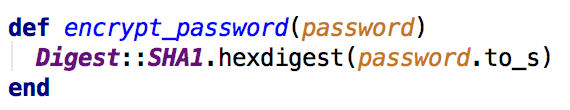
\includegraphics[keepaspectratio=true,scale=0.85]{pictures/encryptpassword.png}}
\captionof{figure}{Szyfrowanie hasła}\label{encryptpassword}
\end{minipage}\\
Autoryzacja ma za zadanie zweryfikować czy dany użytkownik faktycznie ma dostęp do żądanych zasobów. W aplikacji zostało to zrealizowane za pomocą  metody sprawdzającej czy dane o które zapytanie wysłał użytkownik naprawdę do niego należą. Dzieje się to dzięki sprawdzania wartości tokenu, który jest generowany dla każdego użytkownika. Token ten jest unikalny dla każdego użytkownika a jego czas życia ogranicza się do długości sesji. 
\begin{minipage}{\linewidth}
\makebox[\linewidth]{
  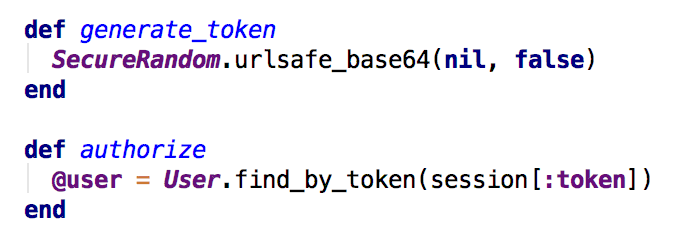
\includegraphics[keepaspectratio=true,scale=0.85]{pictures/authorization.png}}
\captionof{figure}{Autoryzacja za pomocą tokenu}\label{authorization}
\end{minipage}\\
Weryfikacja odbywa się przy każdej metodzie wskazanej w adnotacji before\_action:\\
\begin{minipage}{\linewidth}
\makebox[\linewidth]{
  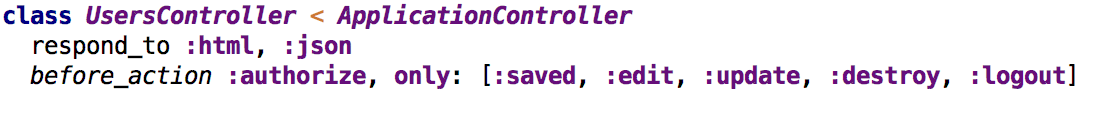
\includegraphics[keepaspectratio=true,scale=0.85]{pictures/beforeaction.png}}
\captionof{figure}{Wskazanie metod, które będą autoryzowane}\label{before_authorization}
\end{minipage}
